% #############################################################################
% This is Chapter Legacy
% !TEX root = ../main.tex
% #############################################################################
% Change the Name of the Chapter i the following line
\fancychapter{Legacy - TODO}
\cleardoublepage
% The following line allows to ref this chapter
\label{chap:conclusion}

% #############################################################################
\section{Hardware Fault Tolerance Mechanisms}
\label{chap2:FTM}



\subsection{Watchdog}
This is a second processor that is used to monitor and ensure proper control flow. Unlike the Lockstep, this isn't a copy of the main CPU; it's a different, much smaller/simple core that observes the main core's interaction with the memory and probes some other deemed crucial signals to verify the overall architecture functioning.



% \subsection{Reduced-Precision Redundancy}
%  This solution bases itself on the previously mention Triple Modular Redundancy (TMR), but aiming to
% improve on it’s performance. As with TMR, three computations are calculated but, to reduce overhead,
% only one with full-precision computing. The remaining two will result on approximate reduced-precision
% values. The three outcomes can still be compared (by voting, as it happens with TMR), but the avoidance of three full-precision computations relieves the core of a significant computational burden, at the
% expense of some result reliability.


% #############################################################################
\section{Choosing the RISC-V ISA}
\label{chap2:risc-v}

This chapter narrows down the baseline architecture that will serve as the hardware foundation for the final \ac{Fatori-V} tool. While \cref{chap2:criteria} details the full set of selection criteria, the first and most significant decision is choosing the \ac{ISA}, which is addressed here. This work assumes a \ac{RISC-V}-based platform. The following paragraphs introduce RISC-V and motivate this choice.

\ac{RISC-V} is a free and open \ac{ISA}, and it is the fifth version of the \ac{RISC} \ac{ISA}. The \ac{ISA} is intentionally modular: a lean base integer subset (RV32I/RV64I) can be extended with optional features such as M (multiply/divide), A (atomics) or C (compressed), allowing designs to scale from minimal microcontrollers to more capable embedded processors.

\begin{figure}[h]
\centering
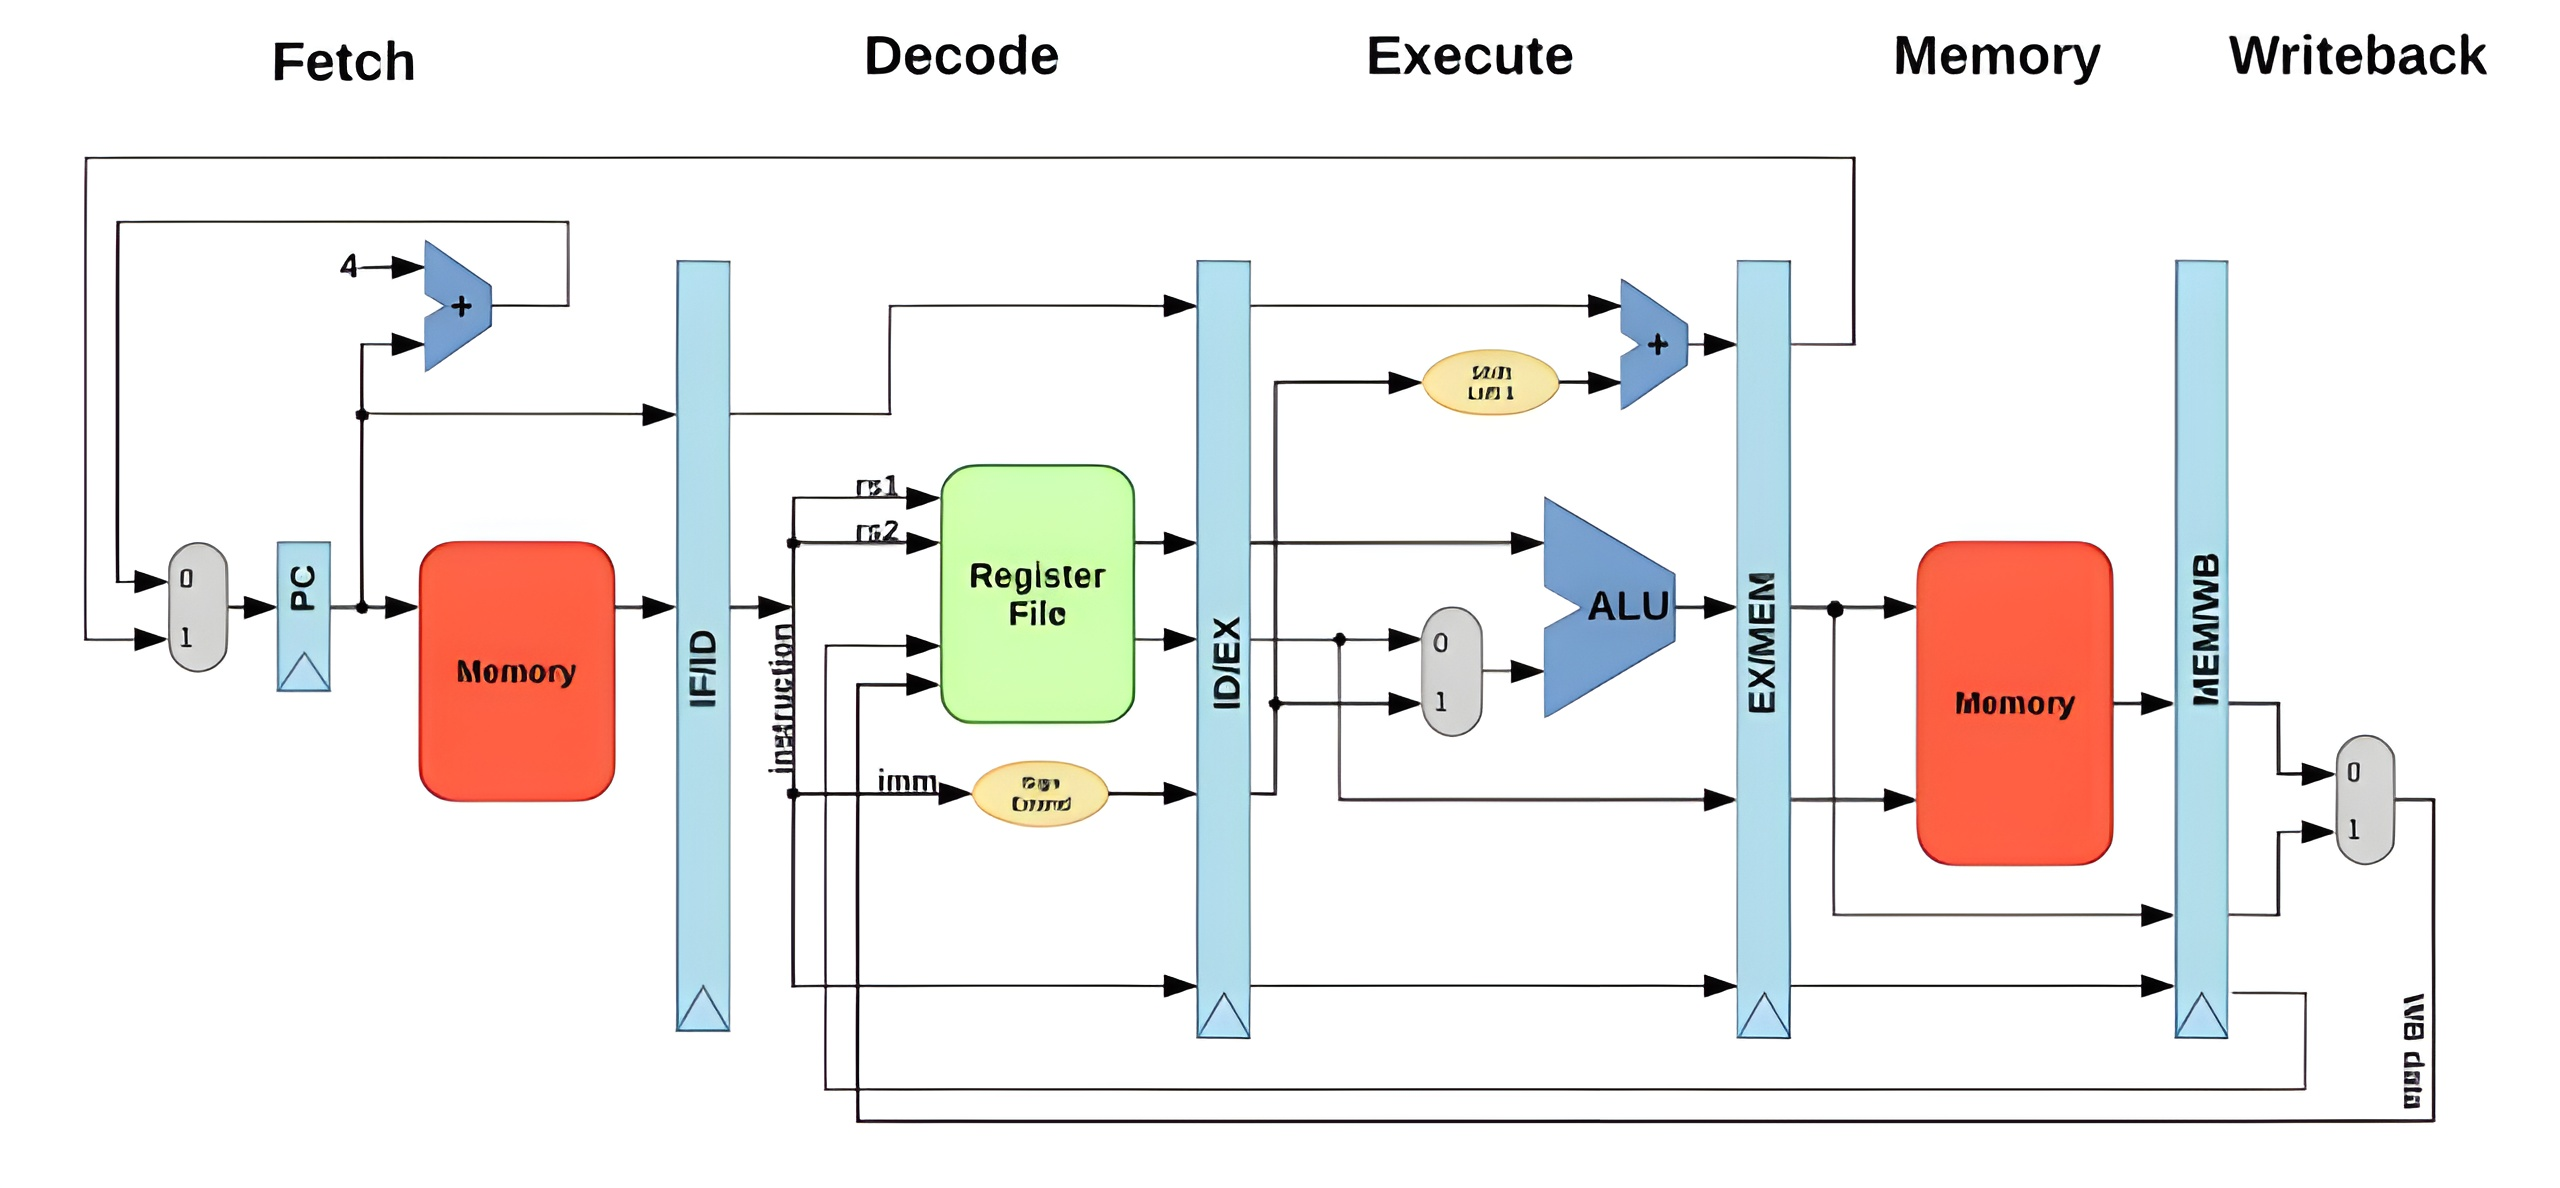
\includegraphics[width=0.75\linewidth]{Images/RiscV_Pipeline.png}
\caption{Example \ac{RISC-V} pipeline.}
\label{fig:riscv_pipeline}
\end{figure}



\Cref{fig:riscv_pipeline} shows a simple 5-stage architecture that can support the \ac{RISC-V} \ac{ISA}, featuring: \ac{IF} (instruction request and next-\ac{PC} computing), \ac{ID} (decode, register read, immediate formation), \ac{EX} (ALU, branch decision), \ac{M} (loads/stores), and \ac{WB} (register write-back). With limited project time, selecting an ISA with an active ecosystem and widely used reference implementations is essential: it reduces integration risk and maximizes the amount of reusable tooling and documentation.




% #############################################################################
\section{Comparative Analysis of the Candidates}
\label{chap2:analysis}

This section summarizes the candidates using the criteria defined in \cref{chap2:criteria}. The comparison reflects an initial survey rather than a deep, uniform evaluation of each platform. Since it relies on published results, the metrics are not always directly comparable across cores (different toolflows, targets, configurations, and benchmark setups). A fully cohesive analysis would require implementing a common baseline integration for each candidate under the same conditions. Nonetheless, this survey provides a consistent enough picture to guide \ac{Fatori-V}'s starting point and reduce early integration risk.

The tables below mix qualitative and quantitative indicators. Documentation is graded on a 0--10 scale (availability of structured manuals, integration notes, onboarding material, and reference documentation). Readability/modification and workflow are expressed as \textit{Very Low} to \textit{Very High} with a short qualifier. \ac{FT} infrastructure is classified as \textit{None}, \textit{Small} (one mechanism), \textit{Medium} (3--4 mechanisms), or \textit{Full} (5+ mechanisms plus a clear error signalling interface). Performance is reported using the best available published metric per core (preferably CoreMark/MHz), and hardware cost uses the most reliable published minimum available (FPGA LUTs or ASIC gate-equivalents, depending on the source).

% --- Table 1/2: (Core + 4 columns) ------------------------------------------
\begin{table}[H]
\centering
\scriptsize
\setlength{\tabcolsep}{3.2pt}
\renewcommand{\arraystretch}{1.18}
\begin{tabularx}{\textwidth}{|l|c|X|X|X|}
\hline
Core &
Documentation (x/10) &
Readability and Modification &
Complete Workflow &
\ac{FT} Infrastructure \\
\hline
\hline
CVA6 &
8 &
Low, complex core &
High, Linux-capable &
Small \\
\hline
CV32E40P &
7 &
High, clean SV &
High, MCU platform &
None \\
\hline
Ibex &
8 &
Very High, modular code &
Medium, simple demo system &
Full*, 8+ \acp{FTM} + \ac{FT} Interface \\
\hline
PicoRV32 &
4 &
Very High, small RTL &
Medium, PicoSoC included &
None \\
\hline
Rocket Chip &
6 &
Very Low, generator heavy &
Very High, Chipyard flow &
Small \\
\hline
VeeR EL2 &
10 &
Medium, SoC coupled &
Very High, custom debbug tools &
Medium*, Data/RF \ac{ECC}, Lockstep \\
\hline
VexRiscv &
6 &
Low, generator workflow &
Medium, many integrations &
None \\
\hline
\end{tabularx}
\caption{Comparison of open-source RISC-V candidates, regarding the most significant criteria (\cref{chap2:criteria}).}
\label{tab:candidate_comparison_fullcriteria}
\end{table}

\begin{table}[H]
\centering
\scriptsize
\setlength{\tabcolsep}{3.2pt}
\renewcommand{\arraystretch}{1.18}
\begin{tabularx}{\textwidth}{|l|c|X|X|c|}
\hline
Core &
Local &
Minimal Hardware Cost (published) &
Maximum Performance (published) &
Community \\
\hline
\hline
CVA6 &
No &
--- &
3.1\,CoreMark/MHz* \cite{CVA6_maxperf} &
High \\
\hline
CV32E40P &
No &
40 kG* (conf V1) \cite{CV32E40P_minhw} &
3.19\,CoreMark/MHz* \cite{CV32E40P_maxperf} &
High \\
\hline
Ibex &
No &
16.85\,kGE* (micro) &
3.13\,CoreMark/MHz* (maxperf) \cite{Ibex_maxperf} &
Very high \\
\hline
PicoRV32 &
Local SoC Implementation &
\(\sim\)750 LUT* (Xilinx 7-series) \cite{PicoRV32_minhw} &
0.40\,CoreMark/MHz* \cite{PicoRV32_maxperf} &
High \\
\hline
Rocket Chip &
No &
--- &
2.108\,CoreMark/MHz* (Rocket) \cite{RocketChip_maxperf} &
Very high \\
\hline
VeeR EL2 &
Previous work &
--- &
3.6\,CoreMark/MHz* \cite{VeeR_EL2_maxperf} &
High \\
\hline
VexRiscv &
Local SoC Implementation &
504 LUT, 505 FF* (small) \cite{VexRiscv_minhw} &
1.57\,DMIPS/MHz* \cite{VexRiscv_maxperf} &
High \\
\hline
\end{tabularx}
\caption{Comparison of open-source RISC-V candidates, regarding least significant criteria (\cref{chap2:criteria}).}
\label{tab:candidate_comparison_fullcriteria_b}
\end{table}


In the tables, values marked with '*' come from specific published configurations and should be interpreted together with their source. This matters because several projects publish multiple named configurations that target different points in the area--performance trade-off (e.g., Ibex’s small/maxperf/opentitan). Consequently, the reported "minimal hardware cost" and "maximum performance" for the same core may correspond to different configuration choices.

The documentation scores reflect more than a repository README: they capture the amount of structured material that directly supports modification and integration (reference manuals, integration notes, verification/bring-up guidance, and guided onboarding). Under this lens, VeeR EL2 stands out by combining reference documentation with unusually extensive guided learning material, including a full architecture course. Ibex benefits from a structured documentation site and “product-like” reference material around configuration and behaviour. Minimalist cores like PicoRV32 contain limited documentation, and generator-based projects (Rocket Chip, VexRiscv) often split documentation across the generator and its integration frameworks, which makes it less centralized.

The readability/modification and workflow columns also capture a structural split: static \ac{RTL} codebases versus generator-driven flows. In practice, embedded SystemVerilog cores with well defined module boundaries (CV32E40P, Ibex) are configurable via a smaller set of human-written \ac{RTL} files, while generator-based cores (Rocket Chip, VexRiscv) are configurable through the generators, and not directly into \ac{RTL}. The “complete workflow” ratings reflect the Chipyard-style  flow and extensive debug tooling (pipeline viewer, code editor IDE, etc) of the Rocket Chip and VeeRwolf EL2 cores, respectively. The other candidates either ship only a core (with integration examples), provide a lighter/partial SoC workflow, or rely on externally developed SoC integrations rather than a native, full build-and-run platform.

Finally, the hardware-cost and performance rows illustrate why the survey avoids over-interpreting absolute numbers. Cost may be reported in ASIC-like units (kGE) or FPGA-specific ones (LUTs/FF), and performance may use different benchmark families (CoreMark/MHz versus DMIPS/MHz), sometimes from upstream documentation and sometimes from third-party studies or thesis reports. These columns are treated as “best available published indicators” rather than directly comparable rankings.





% -------------------------------------------------------------
\subsubsection{Build Workflow and Native Source Generation}
\label{chap5:ibex_buildflow}

 The architecture is organized in three layers, each implemented as a Git submodule of the upper one. The top layer, IOb-SoC-Ibex \cite{iob-soc-ibex}, plays the role of the \ac{SoC} project, and is a modified version of IOb-SoC \cite{iob-soc}. The first change was selecting Ibex as the \ac{CPU} by instantiating the "iob\_ibex" block in \texttt{iob\_soc.py}, by changing the "cpu" entry in the \ac{SoC} parameter dictionary:
\begin{lstlisting}[language=matlabfloz,caption={Portion of the new iob\_soc.py}]
**py_params_dict,
"cpu": "iob_ibex",
"mem_addr_w": 18,
\end{lstlisting}

 With \texttt{"cpu": "iob\_ibex"}, the Py2HwSw flow searches for \textit{iob\_ibex.py} in the project's submodules. For that reason, the second modification was creating IOb-Ibex \cite{iob-ibex} as a submodule and providing its Python description file.

 Since IOb-SoC-Ibex is the top of the whole system, it is also where the Vivado \texttt{.tcl} scripts and the firmware executed on the \ac{FPGA} are defined. The intent here was not to develop new benchmarks or custom \texttt{.tcl} scripts permanently inside the \ac{SoC} project, but to create hook points that allow an external upper layer (later, \ac{Fatori-V}) to inject them dynamically. Two hook mechanisms were implemented.

 \underline{\texttt{.tcl} probes:} the standard \textit{build.tcl} used by Py2HwSw is normally taken from the framework libraries. In IOb-SoC-Ibex, a modified \textit{build.tcl} was added to introduce a custom sourcing procedure that can include user-provided \texttt{.tcl} files at fixed stages of the Vivado flow while preserving the original script context. The supported stages are: \textit{pre\_synthesis.tcl}, \textit{post\_opt.tcl}, \textit{post\_route.tcl}, \textit{pre\_bitstream.tcl}, and \textit{post\_bitstream.tcl}. The hook directory is provided through the new \texttt{VIVADO\_INPUT} main Makefile argument. The custom sourcing function is shown below:
\begin{lstlisting}[language=matlabfloz,caption={Custom TCL function to source hook probes}]
# Helper procedure to source probes with proper context
proc source_probe {probe_dir probe_name} {
    if {$probe_dir == ""} {
        return
    }

    set probe_file "${probe_dir}/${probe_name}"
    if {[file exists $probe_file]} {
        # Make build.tcl variables available to probes
        global NAME CSR_IF BOARD #... plus all other variables
        global PROBE_DIR
        set PROBE_DIR $probe_dir
        source $probe_file

        puts ">>> ${probe_name} complete!"
    } else {
        puts ">>> Probe not found: ${probe_file} (skipping)"
    }
}
\end{lstlisting}

 \underline{External benchmark inclusion:} by default, IOb-SoC \cite{iob-soc} builds and runs only the firmware located at \texttt{software/src/iob\_soc\_firmware.c}, which corresponds to the standard Hello World program. In IOb-SoC-Ibex, both the software Makefiles and the firmware wrapper were modified so that an external benchmark can be compiled and executed when a Makefile argument is provided. If the new \texttt{BENCHMARK\_DIR} argument is set, the build system sources the benchmark from that directory; otherwise, it falls back to the default Hello World path. The relevant portion of \textit{sw\_build.mk} (one of the software Makefiles) is shown next:
\begin{lstlisting}[language=matlabfloz,caption={Portion of the new sw\_build.mk}]
#========================================
# Benchmark Configuration
#========================================
ifdef BENCHMARK_DIR
    # External benchmark mode
    BENCHMARK_SRC_DIR = $(BENCHMARK_DIR)
    $(info Building with external benchmark: $(BENCHMARK_DIR))
else
    # Default mode - use hello_world
    BENCHMARK_SRC_DIR = src/hello_world
    $(info Building with default benchmark: Hello World)
endif

#========================================
# BENCHMARK SOURCES
#========================================
# Include benchmark directory in search path (for benchmark.h, port headers)
IOB_SOC_INCLUDES += -I$(BENCHMARK_SRC_DIR)

# If benchmark has a code/ subdirectory, include it and source from it
ifneq ($(wildcard $(BENCHMARK_SRC_DIR)/code/.),)
    BENCHMARK_CODE_DIR = $(BENCHMARK_SRC_DIR)/code
    IOB_SOC_INCLUDES += -I$(BENCHMARK_CODE_DIR)
    IOB_SOC_FW_SRC += $(wildcard $(BENCHMARK_CODE_DIR)/*.c)
    $(info   Including prepared code from: $(BENCHMARK_CODE_DIR))
endif
\end{lstlisting}

 On the firmware side, the wrapper now includes \texttt{benchmark.h} and calls the benchmark entry point through \texttt{BENCHMARK\_MAIN()}:
\begin{lstlisting}[language=matlabfloz,caption={Portion of the new iob\_soc\_firmware.c}]
uart_puts("=== Running Benchmark ===\n\n");
result = BENCHMARK_MAIN();
\end{lstlisting}

 The only requirement imposed on an external benchmark directory is the presence of a \texttt{benchmark.h} header that defines the entry point macro and optional metadata. For example, CoreMark exposes:
\begin{lstlisting}[language=matlabfloz,caption={Portion of Coremark's benchmark.h}]
// Entry point function - called by wrapper
extern int coremark_main(void);

// Benchmark metadata
#define BENCHMARK_MAIN    coremark_main
#define BENCHMARK_NAME    "CoreMark"
\end{lstlisting}

 These two hook points (\texttt{.tcl} probes and external benchmark selection) are later used by the \ac{Fatori-V} software layer to generate \texttt{.tcl} scripts and to run user-selected benchmarks, as described in \cref{chap7:fatori_software}.

 Finally, because Ibex is SystemVerilog-based and relies on package compilation order, the FPGA Makefile was adjusted so that \texttt{*\_pkg.sv} files are compiled before other \texttt{.sv} and \texttt{.v} sources that import them. This change was implemented in the top layer under \texttt{hardware/fpga/Makefile}:
\begin{lstlisting}[language=matlabfloz,caption={Portion of the new hardware/fpga/Makefile (source ordering)}]
#include the module's headers and sources
VHDR+=$(wildcard ../src/*.vh) $(wildcard ./src/*.vh)
PCKS+=$(wildcard ../src/*_pkg.sv)
VSRC+=$(PCKS)
SVRC+=$(wildcard ../src/*.sv)
VSRC+=$(filter-out $(PCKS), $(SVRC))
VSRC+=$(wildcard ../src/*.v) $(wildcard ./src/*.v)
VHDR+=$(wildcard ../common_src/*.vh)
VSRC+=$(wildcard ../common_src/*.v)
\end{lstlisting}

\vspace{2mm}
The second layer, IOb-Ibex \cite{iob-ibex}, is responsible for making the Ibex \ac{RTL} available to the Py2HwSw build directory in a controlled and updatable way. Py2HwSw copies into the build directory whatever exists under \texttt{iob\_ibex/hardware/src/}, but Ibex is composed of many source files. Copying the full native Ibex tree into IOb-Ibex would both bloat the repository and freeze it in time. The approach taken was to keep locally modified or integration-specific files in \texttt{hardware/src/}, while native Ibex \ac{RTL} files are generated and copied in when needed. IOb-Ibex's main Makefile uses Ibex's native repository to generate the source files (see bellow) and copies them directly into the build directory while explicitly excluding any file for which a locally modified version already exists in \texttt{hardware/src/}. This ensures that local fixes and extensions are not overwritten by generation. The last modification of this layer comes from the fact that the Ibex \ac{RTL} is SystemVerilog-based. Py2HwSw commonly generates a Verilog wrapper \texttt{iob\_ibex.v} from \texttt{iob\_ibex.py}, but the Ibex sources that follow require SystemVerilog. For that reason, \texttt{iob\_ibex.py} disables the automatic HDL generation by setting \texttt{"generate\_hw": False}, and the actual wrapper is provided manually as \texttt{iob\_ibex.sv} under \texttt{hardware/src/}. Even with generation disabled, \texttt{iob\_ibex.py} remains required because Py2HwSw still parses it to understand the module interfaces and to derive system parameters such as clock and UART settings (for example, BAUD and frequency-related configuration).
 
The third layer contains the official Ibex repository \cite{ibex}, included as a submodule of IOb-Ibex. The purpose of this layer is to provide a source for the generation Makefile targets of the previous layer. The official Ibex repository provides \textit{make} and FuseSoC-based targets that can generate a complete SystemVerilog-based set of \ac{RTL} source files. IOb-Ibex uses these targets to export the necessary files and dependencies, and then copies the generated outputs into the Py2HwSw project structure. The main difficulty was creating a way to run these targets without manually installing and maintaining all tool dependencies. Py2HwSw-based projects use Nix Environments to manage dependencies, which would be a good solution to the problem, but the required packages were not compatible with these Nix Environments. The solution was to include Ibex-Demo-System \cite{ibex-demo-system} (the officially provided Ibex's example implementation) in the third layer, also as a submodule of IOb-Ibex. This new repository provides a Nix Flakes environment, a more recent approach to Nix Environments, that already contains the dependencies needed for the Ibex generation flow. IOb-Ibex's generation targets enter the demo system's \cite{ibex-demo-system} nix-shell and, from there, run the required FuseSoC commands in the official Ibex repository \cite{ibex}.



 % -------------------------------------------------------------
\subsection{Py2HwSw Infrastructure}
\label{chap5:py2hwsw}

Py2HwSw \cite{py2hwsw} is a Python framework for embedded hardware/software design that generates a complete tool-ready \ac{RTL} project from a short Python system description.\\
In a Py2HwSw project, the user describes the system in Python, typically through a small set of \textit{.py} entry files that declare which modules exist, how they connect, and which configuration parameters are active. The platform then creates a self-contained build directory containing collected and generated \ac{RTL} sources, software support, scripts, and Makefiles required for emulation, simulation, synthesis, and \ac{FPGA} bitstream generation/programming. The flow uses open-source tools, and it targets generation of lint-friendly and portable Verilog code that can be used across FPGA and ASIC flows. Projects such as IOb-SoC \cite{iob-soc} follow this model and are an example of a Py2HwSw-based system.

The workflow is organized around three directories:

The \underline{main directory} is the user repository. It contains the Python description, project-specific hardware and software sources, and any overrides to the default infrastructure. This directory is where development changes are applied.

The \underline{Py2HwSw directory} is the framework installation. It provides a reusable library of modules, reference templates, scripts, and build infrastructure. This library allows users to omit implementation blocks in their main directories since the platform will default omissions to Py2HwSw's source files. For example, a system can include a UART connection just by instantiating one in the \textit{.py} description, without actually providing its implementation. The framework will ensure that the relevant Verilog modules are sourced.

The \underline{build directory} is a generated output folder created outside the main repository. It merges the user-provided contents of the main directory and its declared submodules, with the defaults from the Py2HwSw library, resulting in a complete set of sources and Makefiles required to run the supported flows. It can be deleted and regenerated by rerunning setup. After generation, it can also be used as a standalone build workspace, provided the required tools are available.

The Py2HwSw library, as mentioned, exists so that a project can pull in standard building blocks by declaring them in Python. It includes bus infrastructure and converters (covering AXI-family variants and bridges to other common internal buses), memory-oriented components (RAM/ROM-style blocks and register-file style blocks), FIFO variants (including clock-domain-crossing versions), and a set of common peripherals (e.g., UART, timers, GPIO, SPI, DMA-style blocks), alongside scripts/Makefile entry points for running supported flows.

The ecosystem is designed around multiple selectable simulators (icarus, verilator, vcs, questa and xcelium) and board targets (iob\_aes\_ku040\_db\_g [Kintex UltraScale+], iob\_zybo\_z7 [Zynq-7000], iob\_basys3 [Artix-7], iob\_cyclonev\_gt\_dk [Cyclone V], and others). A Nix-based environment is used to make the toolchain reproducible, without having to install dependencies. A preliminary user guide is provided by the project and is maintained in LaTeX, with a Makefile target to build it.


% -------------------------------------------------------------
\subsection{Features Summary}
\label{chap3:features}

 \ac{Fatori-V} packs many features that, unfortunately, this report does not have space for. This section serves to list most of them in order to provide the user with a better understanding of the capabilities of the system.\\\\
Architecture configuration (per run)
\begin{itemize}
    \item Enable/disable performance features (e.g., instruction cache, branch predictor, writeback stage, branch-target ALU) with simple on/off switches.
    \item Enable/disable ISA extensions (e.g., RV32M/RV32C/RV32B variants) and select implementation variants (e.g., multiplier style, regfile style).
    \item Select the metrics “depth”/level to trade observability vs. overhead (which dynamically changes the amount of metric counters generated in the \ac{RTL}).
\end{itemize}

 Fault tolerance configuration
\begin{itemize}
    \item Enable/disable \acp{FTM} in the \textit{.yaml} and tune their parameters (including mechanisms that are native to Ibex and those introduced by Fatori-V).
    \item Configure M-of-N redundancy independently per-register and for selected logic blocks (including the number of replicas, minimum quorum, and hold behaviour - see \cref{chap6:mofn_reg} and \cref{chap6:mofn_logic}).
    \item Configure self-test policies and spacing (what to test, when to test, and what to do in the event of failure). See \cref{chap6:self_test}.
\end{itemize}

 Fault injection workflow (see \cref{chap8:fatori_fi}).
\begin{itemize}
    \item Run with or without fault injection while keeping the overall run workflow identical.
    \item Choose where to inject (area profile) and when to inject (time profile), including module-scoped injection and more complex time profiles (uniform/ramp/Poisson/microburst/MMPP2/trace-driven).
    \item Support both configuration-memory (SEM) injection and register injection (via UART protocols) with a unified target abstraction inside the FI engine.
\end{itemize}

 Batch execution and automation
\begin{itemize}
    \item Place multiple \textit{.yaml} files in runs/ and execute them sequentially, with automatic separation of outputs per run.
    \item Choose a dry-run/debug mode that performs validation, generation, file movement, and command construction without actually executing the commands or injecting faults (useful for development or when hardware is unavailable).
    \item Produce deterministic runs using explicit seeds for the reproducibility of generation and injection behaviour.
    \item Add custom incompatibility checks and subsequent corrections to the centralized validation system so that, during the validation phase, the system automatically identifies and corrects them.
    \item Execute multiple benchmarks sequentially (with in-between system resets) on the same architecture. Additionally, new benchmarks and their respective configuration inputs can be easily added to the \textit{.yaml} run files, and the system will automatically recognize them.
\end{itemize}

 Traceability and reporting
\begin{itemize}
    \item Store per-run logs and per-session logs automatically.
    \item Configure the exact messages you want to appear in each log event (the actual string being shown) in a centralized logging system.
    \item Run the system with one of three log levels (minimal, normal, or verbose), which you can adjust at will: choose which events are logged in each log level.
    \item Export consolidated results tables (.csv and .xlsx) that merge benchmark metrics with FPGA build metrics (directly parsed from Vivado reports).
    \item Mirror generated files and build reports into the results folder to make runs reproducible later.
    \item Add new indirect metrics (computed from metrics that are directly measured) by simply adding a new formula in a centralized \textit{config} file. These new results will automatically appear in the results tables.
\end{itemize}


% -------------------------------------------------------------
\subsection{Native Fault Tolerance Mechanisms}
\label{chap5:ibex_ftm}

When looking deeper into Ibex’s built-in \acp{FTM}, it becomes clear that most of them target deliberate attacks rather than natural \acp{SEU}, often by adding randomness or reducing timing and power predictability. Despite not aligning exactly with \ac{Fatori-V}'s main goal, these mechanisms are still relevant and will be included in the final \ac{FTM} analysis for comparison. The following subsections describe the native \acp{FTM} present in Ibex and identify which parts are directly useful for \ac{Fatori-V}.

\subsubsection{Data Independent Timing}
When enabled, execution times and power consumption of all instructions are independent of input data. This makes it more difficult for an external observer to infer secret data by observing power lines or exploiting timing side-channels.\\
When data-independent timing is enabled: branches execute identically regardless of their taken/not-taken status; early completion of multiplication by zero/one is removed; early completion of divide by zero is removed;

\subsubsection{Dummy Instructions}
 This mechanism inserts dummy instructions at random intervals into the execution pipeline. The dummy instructions have no functional impact on processor state, but add some difficult-to-predict timing and power disruption to executed code. This disruption makes it more difficult for an attacker to infer what is being executed, and also makes it more difficult to execute precisely timed fault injection attacks. This is not a mechanism specifically designed for space shielding, but is very useful against side-channel attacks, and can still be found in many Fault Tolerant Systems.

\subsubsection{Hardened PC}
 The program counter and branch logic are high-impact hardware modules. During sequential flow, the current \ac{IF}'s \ac{PC} must equal the previous \ac{PC} plus the expected increment (2 or 4 bytes if the C extension is enabled, otherwise 4). A check is set, and any mismatch raises an internal major alert, preventing wild branches at modest cost and without interfering with legitimate control-flow changes.

\subsubsection{Shadow CSRs}
 Certain critical \acp{CSR} (mstatus, mtvec, cpuctrl, pmpcfg and pmpaddr) have extra glitch detection enabled. This creates a second copy of the register that stores a complemented version of the main \ac{CSR} data. A constant check is made to ensure that the two copies are consistent, and an internal major alert is signaled if they are not.

\subsubsection{Dual Core Lockstep}
 This mechanism instantiates a second copy of the core logic, referred to as the shadow core. The shadow core executes using a delayed version of all inputs supplied to the main core. All outputs of the shadow core are compared against a delayed version of the outputs of the main core. Any mismatch between the two sets of outputs will trigger an internal major alert.

\subsubsection{ICache Error Correcting Code}
 \ac{ECC} appends parity bits to a data word so that single-bit errors can be corrected and double-bit errors detected (for example, \ac{SECDED}). An algorithm (like Hamming Codes) is executed, which generates parity bits from the actual data. Both the data and the parity bits are stored together. Upon reading, the system reruns the same algorithm and compares its outcome with the stored parity.\\
Overheads include extra bits per word and encode/decode logic that may add a small pipeline latency.\\\\
It is one of the most commonly used techniques to protect memories. Natively, Ibex provides optional \ac{ECC} protection to the ICache.

\subsubsection{Bus Integrity Checking}
 Extra signals are available alongside the instruction and data side memory channels to support bus integrity checking. When enable, incoming data will be checked against the supplied checkbits. An internal interrupt will be generated and a bus major alert signalled if there is a mismatch. 


 % #############################################################################
\section{PBlock Assignment Model}
\label{chap7:pblock}

To use \ac{ACME}-style spatial aiming (\cref{chap8:fi_acme_impl}), requests such as "inject into the \ac{ALU}", require the target (the \ac{ALU} in this example) to be mapped into fixed physical regions because \ac{SEM}/\ac{ACME} only injects on configuration-memory addresses tied to \ac{FPGA} coordinates, and the \ac{FI} system needs to know which coordinates belong to that target. \ac{Fatori-V} therefore constrains each targetable hardware module to a dedicated pblock with known slice bounds. Because Ibex and the surrounding infrastructure can vary significantly in size across different configurations (\ac{ISA} options, caches, branch logic, RV32B/RV32M choices, \ac{FI} mode, selected \acp{FTM}, and the number of hardware monitors selected), pblock dimensions must be computed dynamically for each run. This section describes the sizing model formulation, the empirical study conducted to characterize the model's constants, and the automated implementation that generates pblocks for arbitrary configurations.

For this first version of \ac{Fatori-V}, the Pblock Model sizes pblocks for these selected targets: ALU, LSU, CONTROLLER, DECODER, MULTDIV (multiplier), BRANCH\_PREDICT (branch predictor), FAULT\_MGR (fault manager) and the SystemVerilog pipeline stage blocks IF\_STAGE, ID\_STAGE and WB\_STAGE.

% -----------------------------------------------------------------------------
\subsection{Pblock Sizing Model}
\label{chap7:pblock_sizing_model}

The general sizing equation for any pblock target is assumed, at this stage, to be:

\begin{equation}
\begin{aligned}
\text{Pblock}_{\text{target}} = \Bigg[ & \Big( B_{\text{target}} \times \prod F_i  - \sum_{\text{child}} B_{\text{child}} + \sum S_{\text{additive}} + \sum R_{\text{target}} \\
&  + \sum_{\text{child}} \text{Pblock}_{\text{child}} \Big) \times \text{MON}_{\text{logic}}(N_{\text{target}}) + S_{\text{MoN}}\Bigg] \times M_{\text{target}}
\end{aligned}
\label{eq:pblock_general}
\end{equation}

Baseline size ($B_{\text{target}}$) is the measured \ac{LUT} count for a module with all optional features and \acp{FTM} disabled. For composite targets (targets that include targets), the baseline includes all child modules at their baseline sizes. Some modules have multiple implementations with different baselines (e.g., different multiplier variants selected by RV32M mode).

Feature factors ($F_i$) are multiplicative scaling factors representing architectural features that restructure module internals. Examples include RV32B bitmanip extension for the \ac{ALU} (which transforms the entire datapath) or ICACHE for IF\_STAGE (which replaces the prefetch buffer with a fundamentally different architecture). Modules unaffected by a particular feature use $F=1.0$, and multiple features compose multiplicatively.

Logic replication factor ($\text{MON}_{\text{logic}}(N)$ is the scaling factor when a module is replicated $N$ times for M-of-N fault tolerance. Only modules with logic-level MON wrappers (\ac{ALU}, CONTROLLER, DECODER, IF\_STAGE, \ac{LSU}) can be logically replicated; others use $\text{MON}_{\text{logic}}(1) = 1.0$. At this stage, this overhead is assumed to scale multiplicatively with $N$, but may also include additive overhead ($S_{\text{MON}}$).

Register replication overhead ($R_{\text{module}}$) is the \ac{LUT} cost for using M-of-N in the registers. Each module contributes:
\begin{equation}
R_{\text{module}} = N_{\text{regs,module}} \times \text{MON}_{\text{reg}}(N_{\text{module}}) \times k_{\text{reg}}
\label{eq:register_component}
\end{equation}
where $N_{\text{regs,module}}$ is the number of FATORI\_REG instances in the module, $\text{MON}_{\text{reg}}(N)$ is the register-level M-of-N overhead function, and $k_{\text{reg}}$ is the per-register \ac{LUT} cost.

Additive components ($S_{\text{additive}}$) are fixed-size independent scaling factors added to the target. The model uses multiplicative factors when features restructure module internals and additive terms when features add independent interface logic or external blocks.

Composite target handling ($\sum_{\text{child}} \text{Pblock}_{\text{child}}$) is needed because child modules are sized recursively using their own pblock equations with their specific feature factors and replication settings preventing double-counting.

Safety margin ($M_{\text{target}}$) is a multiplicative margin applied to the entire pblock size to account for routing overhead and placement constraints.

\Cref{tab:pblock_model} applies this general equation to each possible pblock target. The formulas shown represent initial assumptions combining both multiplicative and additive terms where features could plausibly scale either way. To assign values to all the factors, an empirical study was conducted and is described in the next sections.

\begin{table}[htbp]
\centering
\caption{Pblock sizing equations per target, derived from \cref{eq:pblock_general}.}
\label{tab:pblock_model}
\setlength{\tabcolsep}{4pt}
\scriptsize
\renewcommand{\arraystretch}{1.4}
\begin{tabularx}{\linewidth}{@{}lp{6cm}X@{}}
\toprule
Target & Formula & Observations \\
\midrule
ALU & $[( B_{\text{ALU}} \times F_{\text{RV32B}} + S_{\text{MULTDIV}}) \times \text{MON}_{\text{logic}}(N_{\text{ALU}}) \quad +$ & RV32B significally alters the composition of the ALU. MULTDIV\\
& $ S_{\text{MON}}] \times M_{\text{ALU}}$ &  integration and MON may add fixed costs. \\
\midrule
LSU & $\left[ (B_{\text{LSU}} + R_{\text{LSU}})  \times \text{MON}_{\text{logic}}(N_{\text{LSU}}) + S_{\text{MON}} \right] \times M_{\text{LSU}}$ & Contains FATORI\_REG instances and MON. \\
\midrule
CONTROLLER & $[ (B_{\text{CTRL}} + S_{\text{WB}} + R_{\text{CTRL}}) \times \text{MON}_{\text{logic}}(N_{\text{CTRL}}) \quad +$ & Contains FATORI\_REG instances and MON. The WBSTAGE, when \\
& $S_{\text{MON}}] \times M_{\text{CTRL}}$ & enabled, adds some control logic. \\
\midrule
DECODER & $[ (B_{\text{DEC}} + S_{\text{RV32B}} + S_{\text{WB}} + R_{\text{DEC}}) \times \text{MON}_{\text{logic}}(N_{\text{DEC}}) \quad +$& RV32B adds contained decode logic. The WBSTAGE, when \\
&$ S_{\text{MON}} ] \times M_{\text{DEC}}$ & enabled, adds some decode logic. \\
\midrule
IF\_STAGE & $[ (B_{\text{IF}} \times F_{\text{ICACHE}} + S_{\text{BP}} \, \{- B_{\text{PBuff}} + \text{Pblock}_{\text{PBuff}} \}+ R_{\text{IF}}) \, \times$ & ICACHE and the Prefetch Buffer are mutually exclusive, and both \\ 
& $ \text{MON}_{\text{logic}}(N_{\text{IF}}) + S_{\text{MON}}] \times M_{\text{IF}}$ & significantly alter the composition of the target. The Prefetch Buffer is also a Pblock target, so it must be added as a child. The "\{\}" notation represents optional features. \\
\midrule
ID\_STAGE & $\left[ (B_{\text{ID}} - B_{\text{CTRL}} - B_{\text{DEC}}) + \text{Pblock}_{\text{CTRL}} + \text{Pblock}_{\text{DEC}} \right.$ & Composite target. Contains CTRL and DEC as children. \\
 & $+ S_{\text{BTALU}} + S_{\text{MULTDIV}} + R_{\text{ID}}] \times M_{\text{ID}}$ & BTALU and MULTDIV integration may add fixed interface costs.\\
\midrule
MULTDIV & $B_{\text{MULTDIV}} \times M_{\text{MULTDIV}}$ & Multiple implementations (Slow/Fast/SingleCycle) with distinct \\ & $B_{\text{DSP,MULTDIV}} \times M_{\text{DSP,MULTDIV}}$ & baselines and DSP counts. \\
\midrule
BRANCH\_PREDICT & $B_{\text{BP}} \times M_{\text{BP}}$ & Fixed module instantiated when branch prediction enabled. \\
\midrule
PREFETCH\_BUF & $\left[ B_{\text{PREFETCH}} + R_{\text{PREFETCH}} \right] \times M_{\text{PREFETCH}}$ & Mutually exclusive with ICACHE. Contains FATORI\_REG instances. \\
\midrule
WB\_STAGE & $\left[ B_{\text{WB}} + S_{\text{WSTAGE}} + R_{\text{WB}} \right] \times M_{\text{WB}}$ & WSTAGE adds pipeline logic when enabled. \\
\midrule
FAULT\_MGR & $\left[ B_{\text{FMGR}} + S_{\text{ML}} + R_{\text{FMGR}} \right] \times M_{\text{FMGR}}$ & $S_{\text{ML}}$ is METRIC\_LAYER overhead (instrumentation counters). \\
\bottomrule
\end{tabularx}
\end{table}


% -----------------------------------------------------------------------------
\subsection{PBlock Model Empirical Study}
\label{chap7:pblock_study}

To parameterize the equations in \cref{tab:pblock_model}, a systematic empirical study was carried out across representative hardware configurations. Each configuration contains a controlled subset of parameters while keeping the remaining ones fixed, so that baseline sizes ($B_{\text{target}}$), feature factors ($F$), register overhead ($R$), additive overhead ($S_{additive}$) and  $\text{MON}_{\text{logic}}(N)$/ $\text{MON}_{\text{reg}}(N)$ forms can be extracted. For each configuration, the design was synthesized and implemented on the XCKU040 \ac{FPGA}, and hierarchical utilization reports were parsed to obtain per-module \ac{LUT}/DSP counts. \Cref{tab:pblock_configs} summarizes the full set of configurations, grouped as: (i) baseline characterization, (ii) architectural feature isolation, (iii) logic-level MON replication scaling, (iv) METRIC\_LAYER overhead isolation, (v) interaction validation, and (vi) register-level MON overhead.

\begin{table}[htbp]
\centering
\caption{Systematic empirical characterization configurations.}
\label{tab:pblock_configs}
\setlength{\tabcolsep}{3pt}
\scriptsize
\renewcommand{\arraystretch}{1.15}
\begin{tabularx}{\linewidth}{@{}llX@{}}
\toprule
Config & Group & Configuration and measurement objective \\
\midrule
\multicolumn{3}{l}{\textit{Baseline: Establish $B_{\text{target}}$ for all 11 targets}} \\
C01 & Baseline & All features off: ICACHE/BP/BTALU/WSTAGE=0, RV32B/RV32M=None, \\
 & & MON\_N=1 (all), FAULT\_MGR=0. Measure all 11 baseline LUT counts. \\
\midrule
\multicolumn{3}{l}{\textit{Architectural features: Measure $F$ scaling factors}} \\
C02 & RV32B & RV32B=Balanced. Measure ALU with balanced bitmanip extension. \\
C03 & RV32B & RV32B=OTEarlGrey. Measure ALU with OTEarlGrey bitmanip variant. \\
C04 & RV32B & RV32B=Full. Measure ALU with full bitmanip extension. \\
C05 & RV32M & RV32M=Slow. Measure MULTDIV slow multiplier variant (baseline EX\_BLOCK + slow MULTDIV). \\
C06 & RV32M & RV32M=Fast. Measure MULTDIV fast multiplier variant (baseline EX\_BLOCK + fast MULTDIV). \\
C07 & RV32M & RV32M=SingleCycle. Measure MULTDIV single-cycle variant (baseline EX\_BLOCK + single-cycle MULTDIV). \\
C08 & Cache & ICACHE=1 (PREFETCH=0). Measure IF\_STAGE with instruction cache vs baseline prefetch buffer. \\
C09 & Branch & BRANCH\_PRED=1. Measure IF\_STAGE with branch predictor overhead. \\
C10 & Branch & BRANCH\_TALU=1. Measure ID\_STAGE with branch target ALU overhead. \\
C11 & Writeback & WSTAGE=1. Measure WB\_STAGE presence (vs merged writeback in 2-stage pipeline). \\
\midrule
\multicolumn{3}{l}{\textit{MON logic replication: Determine $\text{MON}_{\text{logic}}(N)$ functional form}} \\
C12 & MON & CONTROLLER: MON\_N=3, MON\_M=2. Test CONTROLLER replication scaling. \\
C13 & MON & CONTROLLER: MON\_N=5, MON\_M=3. Validate CONTROLLER scaling at higher N. \\
C14 & MON & DECODER: MON\_N=3, MON\_M=2. Test DECODER replication (check for anomalous scaling). \\
C15 & MON & DECODER: MON\_N=5, MON\_M=3. Validate DECODER scaling at higher N. \\
C16 & MON & ALU: MON\_N=3, MON\_M=2. Test ALU replication scaling (reference module). \\
C17 & MON & ALU: MON\_N=5, MON\_M=3. Validate ALU scaling at higher N. \\
C18 & MON & LSU: MON\_N=3, MON\_M=2. Test LSU replication scaling. \\
C19 & MON & LSU: MON\_N=5, MON\_M=3. Validate LSU scaling at higher N. \\
C20 & MON & IF\_STAGE: MON\_N=3, MON\_M=2. Test IF\_STAGE replication scaling. \\
C21 & MON & IF\_STAGE: MON\_N=5, MON\_M=3. Validate IF\_STAGE scaling at higher N. \\
C22 & MON & MULTDIV: MON\_N=3, MON\_M=2 (with RV32M=Fast). Test MULTDIV replication scaling. \\
C23 & MON & MULTDIV: MON\_N=5, MON\_M=3 (with RV32M=Fast). Validate MULTDIV scaling at higher N. \\
C24 & MON & All six modules: MON\_N=2, MON\_M=1. Quick validation point for N=2. \\
\midrule
\multicolumn{3}{l}{\textit{METRIC\_LAYER: Measure $S_{\text{ML}}$ and the Metrics Level overhead}} \\
C25 & Metrics & FAULT\_MGR=1, metrics\_level=0 (no HPMC, no FT\_LAYER). Measure FAULT\_MGR baseline. \\
C26 & Metrics & FAULT\_MGR=1, metrics\_level=1 (HPMC only, no FT\_LAYER). Measure HPM overhead. \\
C27 & Metrics & FAULT\_MGR=1, metrics\_level=2 (HPMC + FT\_LAYER\_1). Measure FT\_LAYER\_1 overhead. \\
C28 & Metrics & FAULT\_MGR=1, metrics\_level=3 (HPMC + FT\_LAYER\_1+2). Measure FT\_LAYER\_2 overhead. \\
C29 & Metrics & FAULT\_MGR=1, metrics\_level=4 (HPMC + FT\_LAYER\_1+2+3). Measure FT\_LAYER\_3 overhead. \\
C30 & Metrics & FAULT\_MGR=1, metrics\_level=5 (HPMC + all FT\_LAYERS). Measure FT\_LAYER\_4 overhead. \\
C31 & Metrics & FAULT\_MGR=0, metrics\_level=5. Validate METRIC\_LAYER overhead isolation: \\
 & & with manager disabled, pblock targets should match baseline despite metrics\_level=5. \\
\midrule
\multicolumn{3}{l}{\textit{Interaction validation: Confirm independent scaling}} \\
C32 & Combined & RV32B=Balanced + ICACHE=1. Test independent feature composition on different targets. \\
C33 & Combined & RV32B=Full + ALU:MON\_N=3. Test feature$\times$replication multiplicative composition. \\
C34 & Combined & RV32B=Full + ALU:MON\_N=5. Validate scaling at higher replication with feature enabled. \\
C35 & Combined & ICACHE=1 + BRANCH\_PRED=1 + BRANCH\_TALU=1. Test multiple features on IF\_STAGE and ID\_STAGE. \\
C36 & Combined & RV32B=Balanced + RV32M=Fast + ICACHE=1 + BP=1. Three-way independence test across modules. \\
C37 & Combined & RV32B=Full, RV32M=Fast, ICACHE=1, BP=1, BTALU=1, WSTAGE=1, ALU/LSU:MON\_N=3, \\
 & & FAULT\_MGR=1 + ML=5. Maximum complexity stress test. \\
\midrule
\multicolumn{3}{l}{\textit{Register MON: Measure register replication overhead $R_{\text{target}}$}} \\
C38 & REG\_MON & CONTROLLER: REG\_N=3, REG\_M=2, all registers. Measure replication overhead in moderate-sized module. \\
C39 & REG\_MON & CONTROLLER: REG\_N=5, REG\_M=3, all registers. Validate scaling N=3$\to$N=5. \\
C40 & REG\_MON & IF\_STAGE: REG\_N=3, REG\_M=2, all registers. Measure overhead in register-heavy module. \\
C41 & REG\_MON & IF\_STAGE: REG\_N=5, REG\_M=3, all registers. Validate scaling in large module. \\
C42 & REG\_MON & LSU: REG\_N=3, REG\_M=2, all registers. Cross-validate overhead consistency across modules with similar register counts. \\
C43 & REG\_MON & CONTROLLER + LSU + IF\_STAGE: REG\_N=3, REG\_M=2. Test additive overhead composition across multiple modules. \\
C44 & REG\_MON & CONTROLLER: REG\_N=3, REG\_M=2, 50\% of registers. Test partial coverage scaling \\
C45 & Combined & CONTROLLER: LOGIC\_MON N=3 + REG\_MON N=3. Test interaction between logic and register replication on same module. \\
\bottomrule
\end{tabularx}
\end{table}


% -----------------------------------------------------------------------------
\subsection{Pblock Model Implementation}
\label{chap7:pblock_implementation}

To execute the configurations from \cref{tab:pblock_configs}, \ac{Fatori-V} was used with the override feature enabled. Overriding the auto-generated \texttt{fatori\_pblocks.svh} (which normally disables optimization via \texttt{keep\_hierarchy = true} only for selected \ac{FI} targets) allowed us to stop optimization in every target, for every experiment, to therefore see how each target scales with each feature set. The results in \cref{tab:pblock_results} represent \ac{FI}-enabled overhead with optimization disabled, not production system costs. For actual architecture/\ac{FTM} overhead, see \cref{chap9:results}.

The results of the empirical study (C12--C24, and C38-C45) showed that M-of-N overhead (at both logic and register level) isn't proportional to $N$ (the number of replicas). For $MON_{\text{logic}}$, a fixed $S_{\text{MON}}$ was detected, equal for all modules, because all modules use equal wrapper/voting logic. For register overheads, $MON_{\text{logic}}$ and even $R$, no scaling was detected. This is justified by the fact that optimization blocking is only use for the MON wrapper in logic, and not used at all for register instances, both due to timing issues caused by extreme de-optimization. This will cause smaller pblocks, at the cost of not being able to individually target replicas as \ac{FI} targets.

Metric Level scaling proved localized to non-target modules. Configurations C25--C31 showed that the Fault Manager grows only in \acp{FF} as counter registers are added, with minimal \ac{LUT} increase. The bulk of \ac{CSR} logic (address decode, multiplexers, read/write) resides in the \texttt{cs\_registers} module, which is neither a pblock target nor a child of one, so its scaling does not affect pblock sizing equations.

\Cref{tab:pblock_results} displays both measured target sizes and derived constants. The model implements worst-case sizing: if optimization reduces module sizes below baseline, constants remain at baseline values to guarantee pblocks accommodate all placement scenarios.

\begin{table}[htbp]
\centering
\caption{Empirical pblock sizing study results.}
\label{tab:pblock_results}
\setlength{\tabcolsep}{3pt}
\scriptsize
\renewcommand{\arraystretch}{1.35}
\begin{tabularx}{\linewidth}{@{}p{1.8cm}X p{4.2cm}@{}}
\toprule
Config & Results (\acp{LUT}) & Model Constants \\
\midrule
C01 \newline Baseline & ALU: 238, CONTROLLER: 129, DECODER: 93, IF\_STAGE: 431, LSU: 154, ID\_STAGE: 365, WB\_STAGE: 33, PREFETCH: 168. & $B_{\text{ALU}} = 238$, $B_{\text{CTRL}} = 129$, $B_{\text{DEC}} = 93$, $B_{\text{IF}} = 431$, $B_{\text{LSU}} = 154$, $B_{\text{ID}} = 365$, $B_{\text{WB}} = 33$, $B_{\text{PREF}} = 168$ \\
\midrule
C02--C04 \newline RV32B & C02 Balanced: ALU: 1000, DECODER: +55. \newline C03 OTEarlGrey: ALU: 1772, DECODER: +59. \newline C04 Full: ALU: 2118, DECODER: +56. & $F_{\text{RV32B,None}} = 1.0$, $F_{\text{RV32B,Bal}} = 4.2$, $F_{\text{RV32B,OTE}} = 7.5$, $F_{\text{RV32B,Full}} = 8.9$, $S_{\text{RV32B,Bal}} = 55$, $S_{\text{RV32B,OTE}} = 59$, $S_{\text{RV32B,Full}} = 56$ \\
\midrule
C05--C07 \newline RV32M & C05 Slow: MULTDIV: 621 (0 DSP), ALU: +18, ID\_STAGE: +72. \newline C06 Fast: MULTDIV: 466 (1 DSP), ALU: +17, ID\_STAGE: +71. \newline C07 SingleCycle: MULTDIV: 434 (4 DSP), ALU: +17, ID\_STAGE: +78. & $B_{\text{MULTDIV,Slow}} = 621$, $B_{\text{MULTDIV,Fast}} = 466$, $B_{\text{MULTDIV,Single}} = 434$, $B_{\text{DSP,Slow}} = 0$, $B_{\text{DSP,Fast}} = 1$, $B_{\text{DSP,Single}} = 4$, $S_{\text{MULTDIV,ALU}} = 18$, $S_{\text{MULTDIV,ID}} = 72$ \\
\midrule
C08--C11 \newline Features & C08 ICACHE: IF\_STAGE: 1382. \newline C09 BP: IF\_STAGE: +200, BRANCH\_PREDICT: 38. \newline C10 BTALU: ID\_STAGE: +38. \newline C11 WSTAGE: WB\_STAGE: +4, CONTROLLER: +11, DECODER: +11. & $F_{\text{ICACHE}} = 3.2$, $B_{\text{BP}} = 38$, $S_{\text{BP,IF}} = 200$, $S_{\text{BTALU,ID}} = 38$, $S_{\text{WSTAGE,WB}} = 4$, $S_{\text{WSTAGE,CTRL}} = 11$, $S_{\text{WSTAGE,DEC}} = 11$ \\
\midrule
C12--C24 \newline MON logic & CONTROLLER: +119, DECODER: +117, ALU: +118, LSU: +119, IF\_STAGE: +120. \newline Overhead identical for N=2, N=3, N=5. & $\text{MON}_{\text{logic}}(N) = 1.0$, $S_{\text{MON}} = 120$ \\
\midrule
C25--C31 \newline Metrics & FAULT\_MGR: 1$\rightarrow$5 \acp{LUT}, 1$\rightarrow$114 \acp{FF}. \newline \texttt{cs\_registers} (non-target): +247 (ML=1), +169--359 (ML=2--5). & $B_{\text{FMGR}} = 1$, $S_{\text{ML,max}} = 5$ \\
\midrule
C32--C37 \newline Validation & C37 maximum complexity: ALU\_MON: 2253, MULTDIV: 470, IF\_STAGE: 1735. Feature composition 5--15\% interaction overhead. & $M_{\text{all}} = 1.15$ \\
\midrule
C38--C45 \newline REG MON & CONTROLLER: 125 ($-4$), IF\_STAGE: 424 ($-7$), LSU: 159 (+5). \newline Multi-module C43: $-235$ combined. Overhead identical for N=3, N=5. & $\text{MON}_{\text{reg}}(N) = 1.0$, $R_{\text{module}} = 0$ \\
\bottomrule
\end{tabularx}
\end{table}



% -------------------------------------------------------------
\subsection{AXI Adapter for Ibex}
\label{chap5:ibex2iob}

The IOb-SoC \cite{iob-soc} system uses the AXI protocol to connect its \ac{CPU} to the memory and peripherals, which is a communication interface protocol that moves addresses, data, and responses over five independent channels using a per-channel ready/valid handshake.
The five channels are AW (write address), W (write data), B (write response), AR (read address), and R (read data). On each channel the source asserts X\_VALID, the sink asserts X\_READY, and a transfer occurs in any cycle where both are high. A write presents AW then W and completes when B returns; a read presents AR and later receives data and a response on R. In single-transfer use, burst fields are zero and WLAST=1.

\begin{figure}[H]
\centering
    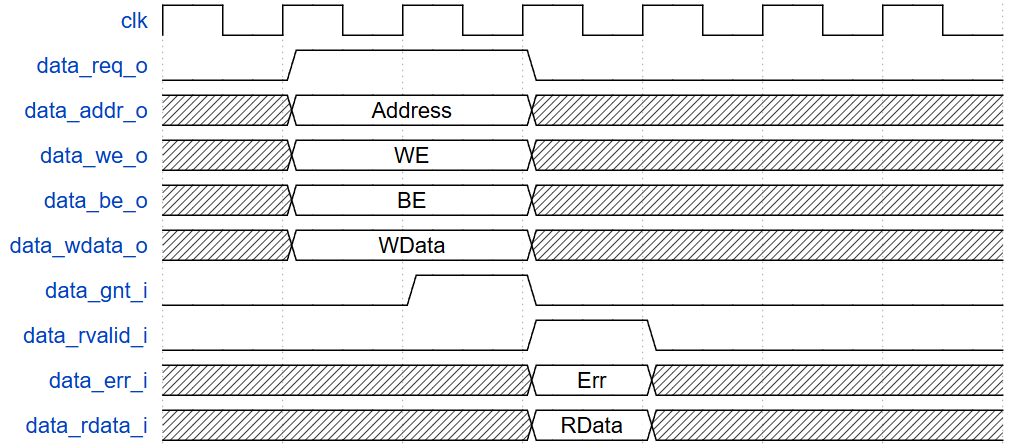
\includegraphics[width=0.8\textwidth]{./Images/Ibex Protocol.png}
    \caption{Ibex \ac{LSU} Interface Timing Diagram }
    \label{fig:ibex_protocol}
\end{figure}

Ibex does not support AXI by origin, instead it uses a request–grant–response system like the one displayed in \cref{fig:ibex_protocol}. To access the memory, the core raises data\_req\_o with data\_addr\_o (stores also raise data\_we\_o) and drives data\_be\_o/data\_wdata\_o. The memory grants with data\_gnt\_i when it has captured the request. Completion is a one-cycle data\_rvalid\_i pulse, carrying data\_rdata\_i for loads and data\_err\_i for errors; responses are in order. To complete the integration, and allow communication with the rest of IOb-SoC (now IOb-SoC-Ibex \cite{iob-soc-ibex}), an AXI-to-Ibex interface module was developed and instantiated at the \ac{CPU}'s wrapper, IOb-Ibex \cite{iob-ibex}, and can be seen in \cref{fig:ibex+iob}. Specification on a set of AXI2Ibex interface signals can be found next, on \cref{tab:axi2ibex}.

\begin{table}[H]
\setlength{\textfloatsep}{3pt}    
\setlength{\intextsep}{3pt}       
\centering
\begin{tabularx}{\textwidth}{|l|X|}
\hline
Signal & Brief explanation \\
\hline
\multicolumn{2}{|l|}{From Ibex (inputs)} \\
\hline
ibex\_*\_req\_i & Requests a memory access; stays high until accepted (load/store on data or instruction fetch). \\
ibex\_*\_addr\_i & Payload address. \\
ibex\_data\_we\_i & Chooses store (high) vs. load (low) on the data path. \\
ibex\_data\_be\_i & Selects which bytes of the aligned word are written. \\
ibex\_data\_wdata\_i & Write payload for stores on the data path. \\
\hline
\multicolumn{2}{|l|}{To Ibex (outputs)} \\
\hline
\textit{ibex\_*\_gnt\_o} & Indicates the request has been captured on the AXI side. \\
\textit{ibex\_*\_rvalid\_o} & One-cycle completion pulse when data/response returns. \\
\textit{ibex\_*\_rdata\_o} & Word returned for loads or instruction fetches. \\
\textit{ibex\_*\_err\_o} & High when the access completes with an error. \\
\hline
\multicolumn{2}{|l|}{To AXI (outputs)} \\
\hline
\textit{*bus\_arvalid\_o} & Validates a read (load or instruction fetch) on the address channel. \\
\textit{*bus\_araddr\_o} & Read address derived from the Ibex. \\
\textit{dbus\_awvalid\_o} & Validates a write on the address channel. \\
\textit{dbus\_awaddr\_o} & Write address derived from the Ibex . \\
\textit{dbus\_wvalid\_o} & Validates a write on the data bus. \\
\textit{dbus\_wdata\_o} & Write data payload sourced from Ibex. \\
\textit{dbus\_wstrb\_o} & Byte strobes selecting which bytes are written. \\
\textit{*bus\_rready\_o}, \textit{dbus\_bready\_o} & Forced ON - always ready to take read data and write responses. \\
\hline
\multicolumn{2}{|l|}{From AXI (inputs)} \\
\hline
\textit{*bus\_arready\_i} & Slave can accept a read address (data or instruction bus). \\
\textit{*bus\_rvalid\_i} & Read data/response is available (data or instruction bus). \\
\textit{*bus\_rdata\_i}, \textit{*bus\_rresp\_i} & Read payload and status code (OK or error). \\
\textit{dbus\_wready\_i} & Slave can accept write data on the data bus. \\
\textit{dbus\_bvalid\_i}, \textit{dbus\_bresp\_i} & Write response and status code on the data bus. \\
\hline
\end{tabularx}
\caption{Snippet of \textit{iob\_ibex2axi}'s interface. Notation: \textit{*bus\_...} expands to both \textit{dbus\_...} and \textit{ibus\_...}; \textit{ibex\_*...} expands to both \textit{ibex\_data\_...} and \textit{ibex\_instr\_...} where applicable.}
\label{tab:axi2ibex}
\end{table}

 For reads (data or instruction), when \textit{ibex\_*\_req\_i} is high with \textit{ibex\_data\_we\_i}=0, the adapter asserts \textit{*bus\_arvalid\_o}. The grant \textit{ibex\_*\_gnt\_o} goes high in the cycle the slave raises \textit{*bus\_arready\_i} while the request is still high. With \textit{*bus\_rready\_o} held high by default, \textit{*bus\_rvalid\_i} produces a one-cycle pulse on \textit{ibex\_*\_rvalid\_o} and the word on \textit{ibex\_*\_rdata\_o}. Upon \textit{*bus\_rresp\_i} detection, \textit{ibex\_*\_err\_o} is asserted.\\
For writes, when \textit{ibex\_data\_req\_i} and \textit{ibex\_data\_we\_i} are high, the adapter asserts \textit{dbus\_awvalid\_o} and \textit{dbus\_wvalid\_o}. The grant \textit{ibex\_data\_gnt\_o} goes high in the cycle the slave raises \textit{dbus\_wready\_i} while the request is still high, after which Ibex may update its request next cycle. With \textit{dbus\_bready\_o} also held high by default, the write response on \textit{dbus\_bvalid\_i} generates a one-cycle \textit{ibex\_data\_rvalid\_o} pulse. \textit{ibex\_data\_err\_o} is asserted on that pulse if \textit{dbus\_bresp\_i} is nonzero.\\
\textit{ibex\_data\_be\_i} is mapped directly to \textit{dbus\_wstrb\_o} and this interface only supports single transfers, so \textit{dbus\_wlast\_o}=1 and unused AXI attributes remain tied to zero.




% -------------------------------------------------------------
\subsection{Per-Experiment \textit{.yaml} File}
\label{chap3:ui_yaml}

 Run files are \textit{.yaml} documents placed in runs/. Each \textit{.yaml} corresponds to one run: it describes the target board, the enabled architectural features and \acp{FTM}, the benchmark sessions to execute, optional fault injection behaviour, and which result artifacts should be preserved. In this section, most configurable fields will be detailed, but not all of them. A complete run file example is available in \cref{app:yaml}.

 Run \textit{.yaml}s are structured into three top-level blocks: run, general, and specifics.

\subsubsection{\textit{Run} Section}
 This section contains general meta information about the experiment itself, not its contents.
\begin{itemize}
    \item run.identification.name \\
    Human-readable run name; used in result folder naming.
    \item run.identification.seed \\
    Seed used to make generation and (where applicable) stochastic decisions reproducible.
    \item run.identification.run \\
    Changes the execution from FPGA targeted to Simulation targeted.
\end{itemize}

\subsubsection{\textit{General} Section}
\label{chap3:yaml_general}
 This section contains on/off switches and high-level choices. This block is meant to remain readable: it answers “what is enabled?” without diving into detailed parameters.\\\\
Features
\begin{itemize}
    \item general.features.fault\_manager \\
    Enables the fault management / extra instrumentation block (commonly used when FI is enabled).
    \item general.features.performance\_mechanisms.* \\
    High-level performance feature toggles like icache, branch\_pred, branch\_target\_alu, wstage;
    \item general.features.isa\_extensions.* \\
    ISA toggles: RV32E, RV32M, RV32B, RV32C;
    \item general.features.fault\_tolerance\_mechanisms.* \\
    High-level FTM toggles: dummy\_instr, lockstep, register\_m\_of\_n, logic\_m\_of\_n, self\_testing, and others;
\end{itemize}

 Benchmarks\\
Configures each benchmark (also called session) that will run in this architecture.
\begin{itemize}
    \item general.benchmarks.\textless bench\textgreater.enable \\
    Enables the benchmark session, disabled benchmarks are skipped.
    \item general.benchmarks.\textless bench\textgreater.config \\
    Benchmark-specific configuration blocks (when applicable), e.g.:
    \begin{itemize}
        \item general.benchmarks.fatori\_stress.config.iterations
        \item general.benchmarks.fatori\_stress.config.targets.\textless module\textgreater
        \item general.benchmarks.embench-iot.config.embench-benchmarks.\textless name\textgreater
    \end{itemize}
\end{itemize}

 Fault injection
\begin{itemize}
    \item general.fault\_injection.enable \\
    Activates \ac{FT} for all enabled benchmarks.
    \item general.fault\_injection.area\_profile \\
    Selects the “where” policy (e.g., whole-device vs module-scoped vs explicit list).
    \item general.fault\_injection.time\_profile \\
    Selects the “when” policy (uniform/ramp/Poisson/etc.).
\end{itemize}

 Metrics and saving behaviour
\begin{itemize}
    \item general.metrics\_level \\
    Accepts a value from 1 to 5 that controls the amount of metric counting hardware included.
\end{itemize}

\subsubsection{\textit{Specifics} Section}
\label{chap3:yaml_specifics}
 This block provides parameters and fine controls for anything enabled in the general section. Most fields are not displayed here due to being too specific.

 Ibex implementation variants
\begin{itemize}
    \item specifics.ibex.*\\
    Specify native Ibex parameters, such as which Register File or Multiplier implementations to use.
\end{itemize}

 Fault tolerance specifics
\begin{itemize}
    \item specifics.fault\_tolerance.reg\_m\_of\_n.* \\
    M-of-N configuration for the registers' implementation:
    \begin{itemize}
        \item N/M selection, seed/percentage policies, hold behaviour
        \item target.\textless module\textgreater selection (choose which module groups are affected)
    \end{itemize}
    \item specifics.fault\_tolerance.logic\_m\_of\_n.* \\
    M-of-N configuration for the logic blocks' implementation:
    \begin{itemize}
        \item N/M selection, hold behaviour, recursive behaviour
        \item target.\textless block\textgreater selection (ALU/decoder/controller/etc.)
    \end{itemize}
\end{itemize}

 Fault Injection detailed profiles
\begin{itemize}
    \item specifics.fault\_tolerance.fault\_injection.time.* \\
    Detailed parameters for each supported time profile (e.g., uniform, ramp, Poisson, microburst, MMPP2, trace, or input), including the injection rate, campaign duration and profile specific arguments.
    \item specifics.fault\_tolerance.fault\_injection.area.* \\
    Detailed parameters for each supported area profile (device/modules/target\_list/input), including:
    \begin{itemize}
        \item target pool sizing 
        \item ratio enforcement (e.g., REG vs CONFIG)
        \item target module selection and optional weights
    \end{itemize}
\end{itemize}

 Pragmatically, the general block decides what is active; the specifics block decides how it behaves. Some of these knobs (such as specifics.fault\_tolerance.reg\_m\_of\_n) directly impact a \textit{.svh} file generation. These sections usually have a *.override field, which accepts a path to an override file that will replace the usually generated one. This can be used for accurate reproducibility or for extremely customized runs.


 % -------------------------------------------------------------
\subsection{Hardware vs Software Layers}
\label{chap3:hwvssw}
 Fatori-V is intentionally split into two layers: the hardware layer (the configurable \ac{SoC} + \ac{FT} improvements) is a RISC-V \ac{SoC} built around Ibex (integrated through IOb-SoC-Ibex and improved for Fatori-V, see \cref{chap5:iob-soc-ibex} and \cref{chap6:fatori_hardware}). Hardware configurability is achieved primarily through compile-time macros: existing modules were extended so that optional features and native \acp{FTM} are gated behind macros, and additional “Fatori modules” were designed from scratch to also accept macro-defined parameters. This approach keeps the underlying architecture stable while allowing the platform to generate many variants without hand-editing \ac{RTL} for each experiment.\\\\
The Software layer, on the other hand, reads the run \textit{.yaml} and turns it into a complete experiment. Concretely, it:
\begin{enumerate}
    \item Validates and normalizes the \textit{.yaml} (applying defaults and compatibility checks defined in the centralized validation system - see \cref{chap7:validation_stage}).
    \item Generates configuration files (see \cref{chap7:generation_stage}), including:
    \begin{itemize}
        \item SystemVerilog headers controlling features and FTMs: fatori\_features.svh, fatori\_ftm.svh, fatori\_reg\_mon.svh, fatori\_logic\_mon.svh, fatori\_selftest.svh, (optionally) fatori\_pblocks.svh and its associated TCL if FI/pblocks are enabled;
        \item Firmware/benchmark configuration headers (e.g., metrics\_config.h, bench\_config*.h)
    \end{itemize}
    \item Allocates generated files into the correct places in the build tree (so the underlying build system compiles the selected design - see \cref{chap7:movement_stage}).
    \item Orchestrates the build and execution of the architecture, synchronizing it with optional FI campaigns (see \cref{chap7:build_stage} and \cref{chap7:execution_stage}).
    \item Collects measurements, performs requested computations, and generates the results tables (see \cref{chap7:results_stage}).
\end{enumerate}

 In this provided snippet of "fatori\_features.svh", the ICache, the Branch Predictor, and the Multiplication ISA extension are enabled; the Write Back Stage, the Bit Manipulation ISA extension, and the Branch Target ALU are disabled.

\begin{lstlisting} [language=matlabfloz,caption={fatori\_features.svh}]
`__FATORI_MACRO_DEF(FATORI_ICACHE, 1)
`__FATORI_MACRO_DEF(FATORI_WSTAGE, 0)
`__FATORI_MACRO_DEF(FATORI_BRANCH_TALU, 0)
`__FATORI_MACRO_DEF(FATORI_BRANCH_PRED, 1)
`__FATORI_MACRO_DEF(FATORI_REGFILE, ibex_pkg::RegFileFPGA)
`__FATORI_MACRO_DEF(FATORI_RV32B, ibex_pkg::RV32BNone)
`__FATORI_MACRO_DEF(FATORI_RV32M, ibex_pkg::RV32MSingleCycle)
\end{lstlisting}

 The “interface” between the layers is therefore simple and robust: the software layer generates files, and the hardware layer consumes them at build time.


 % -------------------------------------------------------------
\subsection{Config and Settings Inputs}
\label{chap3:ui_config}

 Besides run \textit{.yaml}s, Fatori-V relies on two categories of global inputs that are not expected to change from run to run: (1) static input definitions in \texttt{inputs/} and (2) tool customization configuration in \texttt{config/}.

\begin{lstlisting}[basicstyle=\ttfamily\footnotesize,caption={Input and Config files, the entry point of Fatori-V}]
config/
    constants.py
    log_levels.py
    messages_formats.py
    metrics_definitions.py
    validation_checks.py
    Readme
inputs/
    hardware/
        (...)
        locations.yaml
    software/
        (...)
        locations.yaml
    others/
        fatori_registers.yaml
        gen_locations.yaml
        system_hierarchy.yaml
    tcl/
        report_gen.tcl
        sem_gen.tcl
\end{lstlisting}

 The \texttt{inputs/} folder stores static files that directly characterize or influence the architecture and, thus, the execution result. It contains hardware and software code that must not be generated; instead, it is appropriately allocated to a destination at build. The system also allows the user to create its own files and use this as an entry to the system: just add the files to either \texttt{hardware/}, \texttt{software/} or \texttt{others/} and provide the final destination path to locations.yaml (see \cref{chap7:movement_stage}). In \texttt{inputs/others/}, three essential input files are kept from start: \underline{fatori\_registers.yaml} provides a register index organized by module, assigning register IDs and names so that register-related tooling can reference registers consistently (for example, register injection and register wrapper generation workflows); \underline{gen\_locations.yaml} defines a mapping from generated (produced into \texttt{tmp/generated/}) to destination paths inside the hardware/software trees; this is what makes the file movement (“allocation”) phase deterministic and easy to extend when a new generated output is introduced. It uses the same allocation system that the user can use to include new files; \underline{system\_hierarchy.yaml} is used by the system to understand the parent-child relations between logic modules in order to make choices related to recursion; an \texttt{inputs/tcl/} folder is also included here that contains TCL scripts that are either too static or too complex to be generated, such as Vivado report inclusions or IP generation.\\\\
The \texttt{config/} folder defines global platform behaviour. \underline{validation\_checks.py} encodes constraints applied during the validation phase, such as illegal feature combinations, required parameter dependencies, or user-requested compatibilities (see \cref{chap7:validation_stage}). \underline{metrics\_definitions.py} defines what metrics exist, how they are grouped, and how they are computed (either directly measured, or calculated through a formula). \underline{log\_levels.py} and \underline{messages\_formats.py} implement the event-based logging system, where each event has a format definition and each verbosity level decides which events are printed, saved, or both.\\\\
In addition to \texttt{inputs/} and \texttt{config/}, \ac{Fatori-V} has "settings" files scattered through the system. These files contain mostly default values that aren't meant to change, unless something drastically changes (like changing the underlying core in use). The main settings file is \underline{fatori\_settings.py}, which defines default board choices, build strategy (full build per benchmark vs build once + firmware-only runs), clock and baud, and dry-run/debug mode. The most important settings are also \ac{CLI} overridable.

% -------------------------------------------------------------
\subsection{Fatori-V Outputs}
\label{chap3:ui_results}

 Every run creates a dedicated output folder under \texttt{results/\textless run name\textgreater/}.

\begin{lstlisting}[basicstyle=\ttfamily\footnotesize,caption={Results folder, the output of Fatori-V}]
results/
    <run name>/
        gen/
            *.svh
            metrics_config.h
            pblock_config.yaml
            system_dict_merged.yaml
        reports/
            *.rpt
            <board name>_metrics.csv
        sessions/
            bench_metrics.csv
            <benchmark name>/
                gen/
                    bench_config_<benchmark name>.h
                fi/
                    injection_log.txt
                    fi_terminal_log.txt
                fatori_<benchmark name>_log.txt
                metrics.txt
            coremark/
            embench-iot/
            fatori_stress/
            hello_world/
        <run name>.yaml
        verified_yaml.yaml
        <run name>_results_table.csv
        <run name>_results_table.xlsx    
\end{lstlisting}

 At the top level (directly under \texttt{\textless run name\textgreater/}), Fatori-V stores the original run \textit{.yaml}, a verified/normalized \textit{.yaml} (see \cref{chap7:validation_stage}), the consolidated results tables (in CSV and XLS formats) and the terminal dump log files. The \texttt{sessions/} subdirectory stores per-benchmark session data: for each benchmark, the folder includes the benchmark output logs, extracted benchmark metrics (the actual file produced by the firmware running on the FPGA), and (if enabled) \ac{FI} data such as logs and the \ac{FI} system's outputs; additionally, \texttt{sessions/bench\_metrics.csv} provides the benchmark metrics table used later to build the final tables. The \texttt{reports/} subdirectory, when enabled, stores Vivado report files and may include a \texttt{\textless board name\textgreater\_metrics.csv} table summarizing the reports' metrics collected by the report parser. The \texttt{gen/} subdirectory mirrors the exact generated files used for that run, including generated \texttt{.svh} and \texttt{.h} files and intermediate files such as pblock configurations.\\\\
\ac{Fatori-V} produces, as mentioned, consolidated results tables in both CSV and XLSX formats. These merge benchmark metrics (sourced from \texttt{sessions/bench\_metrics.csv}) with \ac{FPGA} build metrics (parsed from Vivado reports into a \texttt{\textless board name\textgreater\_metrics.csv}). The results tables can be considered the main \ac{Fatori-V} output and are exemplified bellow (these are reduced versions).

\begin{table}[H]
\centering
\scriptsize
\setlength{\tabcolsep}{2pt}
\caption{Example and heavily reduced excerpt of the results table (Sheet 1: Benchmark Metrics)}
\renewcommand{\arraystretch}{1.15}
\begin{tabular}{p{0.2\textwidth} p{0.2\textwidth} p{0.2\textwidth} p{0.2\textwidth} p{0.2\textwidth}}
\hline
System Features & FI Parameters & coremark & embench-iot & fatori\_stress\\
\hline
 &  & FI Status: on & FI Status: off & FI Status: off \\

Run Name: example &
FI Corrector: N/A &
instructions\_per\_cycle: 0 &
instructions\_per\_cycle: 0 &
instructions\_per\_cycle: 0 \\

Global Seed: 5432 &
Time Profile: uniform &
detected\_injections: 542 &
detected\_injections: 0 &
detected\_injections: 0 \\

Run Mode: fpga &
Time Seed: uses global &
mcycle: 707200229 &
mcycle: 4837000757 &
mcycle: 11558370 \\

Metrics Level: 5 &
Uniform: Rate Hz: 5.0 &
minstret: 193058420 &
minstret: 1463227089 &
minstret: 2124519 \\

Fault Manager: on &
Uniform: Period s: None &
hpm\_lsu\_busy: 95738778 &
hpm\_lsu\_busy: 490864005 &
hpm\_lsu\_busy: 2423267 \\

Dummy Instructions: off &
Area: Repeat Targets: off &
hpm\_loads: 32646654 &
hpm\_loads: 173880082 &
hpm\_loads: 689186 \\

Logic M-of-N: on &
Area: Seed: uses global &
hpm\_br\_taken: 23406924 &
hpm\_br\_taken: 85672174 &
hpm\_br\_taken: 343518 \\

\hline
\end{tabular}
\label{tab:results_table_benchmark_excerpt}
\end{table}



\begin{table}[H]
\centering
\scriptsize
\setlength{\tabcolsep}{2pt}
\caption{Example and heavily reduced excerpt of the results table (Sheet 2: FPGA Reports)}
\renewcommand{\arraystretch}{1.15}
\begin{tabular}{p{0.16\textwidth} p{0.16\textwidth} p{0.16\textwidth} p{0.16\textwidth} p{0.16\textwidth} p{0.16\textwidth}}
\hline
Common Info & Utilization & Timing & Power & Methodology & DRC \\
\hline
Vivado: v.2020.2 &
Used LUTs: 4678 &
WNS: 2.571 &
OnChip Pw (W): 0.589 &
Metho Violat: 64 &
Violations: 13 \\

Date: Feb 1 2026 &
Total LUTs: 242400 &
TNS: 0.000 &
DPower (W): 0.108 &
SYNTH-15: Warning &
AVAL-318: Warning \\

Design: iob\_aes\_ku040 &
LUTs Util \%: 1.93 &
TNS Fail Endpoints: 0 &
Static Power (W): 0.481 &
SYNTH-15 Desc: ... &
AVAL-318 Desc: ...\\

Dvc: xcku040-fbva676 &
FF Total Used: 2656 &
Total Endpoints: 9849 &
DPower \%: 18.3 &
SYNTH-15 Count: 64 &
AVAL-318 Count: 1 \\

D State: Fully Routed &
Avail FF: 484800 &
WHS: 0.011 &
Static Power \%: 81.7 &
T Warn Viol: 64 &
DPIP-2: Warning \\

 &
DDs Utilization \%: 0.55 &
THS: 0.000 &
 &
 &
DPIP-2 Desc: ... \\

\hline
\end{tabular}
\label{tab:results_table_fpga_excerpt}
\end{table}

% -------------------------------------------------------------
\subsection{Folder hierarchy}
\label{chap3:folder_hierarchy}

 The \ac{Fatori-V} repository is organized by fields.

\begin{lstlisting}[basicstyle=\ttfamily\footnotesize,caption={Fatori-V repository tree}]
Fatori-V/
  architecture/
  benchmarks/
  config/
  fi/
  inputs/
  results/
  runs/
  scripts/
  tmp/
  fatori-v.py
  fatori_settings.py
\end{lstlisting}

 In typical usage, the user primarily edits \texttt{runs/} (run \textit{.yaml} files) and occasionally adjusts static inputs in \texttt{inputs/} and global behaviour in \texttt{config/}.\\
The platform produces one output folder per run under \texttt{results/}, while \texttt{tmp/} is used as a transient workspace during generation and execution. The \texttt{scripts/} folder contains the platform logic organized by subsystems/phases, \texttt{fi/} contains the standalone fault injection engine, and \texttt{architecture/} holds the baseline SoC repository that is configured and built by Fatori-V.\\
The \texttt{benchmarks/} folder, although not a standalone repository in its entirety, is composed of globally used benchmark's repositories and their respective integration ports to this system.


% #############################################################################
\section{Experiments and Results}
\label{chap9:exp_results}

This section reports the experimental results obtained with \ac{Fatori-V}~\cite{FatoriV}.
Results are organised into three groups: Hardware Overhead, Performance, and
Fault Tolerance. The configurations under test span the native Ibex feature set
(\cref{chap5:ibex_features,chap5:ibex_ft}) and the new \acp{FTM} implemented in this work
(\cref{chap6:FTMs}). Only the most relevant metrics are reported in each subsection.

% -----------------------------------------------------------------------------
\subsection{Hardware Overhead}
\label{sec:cost_results}

The first question is how much each protection layer costs in silicon resources. Each
configuration below was synthesised and implemented on the XCKU040 target; LUT, FF, BRAM,
and DSP counts are post-implementation, WNS and dynamic power are from the implementation reports
produced by the build flow (\cref{chap3:ui_results,chap7:results_stage}).

\begin{table}[H]
\centering
\caption{Hardware overhead across baseline, secure, and new-\ac{FTM} configurations.}
\label{tab:cost_results}
\footnotesize
\begin{tabularx}{\textwidth}{lrrrrrr}
\toprule
Configuration & LUTs & FFs & BRAM & DSPs
  & WNS [ns] & Power [W] \\
\midrule
Native Ibex (official SoC)               & 3\,812 & 2\,891 & 4 & 2 & $+1.41$ & 0.74 \\
\ac{Fatori-V} baseline (\texttt{ibex2axi}) & 4\,214 & 3\,108 & 4 & 2 & $+1.19$ & 0.81 \\
Baseline + performance features ON       & 4\,831 & 3\,647 & 8 & 2 & $+0.87$ & 0.93 \\
Secure Ibex (native protections)         & 7\,388 & 5\,821 & 4 & 4 & $+0.61$ & 1.22 \\
Baseline + spatial redundancy (selective)& 6\,073 & 8\,412 & 4 & 2 & $+0.83$ & 1.06 \\
Baseline + self-testing                  & 4\,619 & 3\,441 & 4 & 2 & $+1.08$ & 0.88 \\
Baseline + lightweight checkers          & 4\,902 & 3\,509 & 4 & 2 & $+1.01$ & 0.87 \\
Baseline + all new \acp{FTM} combined    & 8\,247 & 9\,134 & 4 & 4 & $+0.41$ & 1.35 \\
\bottomrule
\end{tabularx}
\end{table}

The dominant cost of spatial redundancy is in FFs (+171\,\% over baseline), not in LUTs,
because \texttt{register\_m\_of\_n} instantiates $N-1$ shadow register files and the associated
majority-voter logic is register-heavy. This is in contrast with \texttt{lockstep}, which
replicates the full pipeline and therefore inflates LUT count roughly equally (+75\,\%) with a
further DSP copy for the multiplier. Lightweight checkers (\texttt{hard\_pc}, \texttt{shadow\_csrs},
\texttt{regfile\_ecc}) add only 688 LUTs and 401 FFs over baseline, confirming the low-cost,
detect-only character of these mechanisms. The WNS degradation trend with increasing replication
depth is expected: voter combinational paths lengthen the critical path, but all configurations
close timing at the target 100~MHz.

% -----------------------------------------------------------------------------
\subsection{Performance}
\label{chap9:perf_results}

Performance is not the primary focus of this thesis, but quantifying the penalty of each
protection layer is necessary to avoid confounding fault-coverage results with execution-speed
effects. The following values are averaged across the CoreMark and Embench-IoT benchmark suite
(\cref{chap7:benchmarks}).

\begin{table}[H]
\centering
\caption{Performance results across baseline, secure, and new-\ac{FTM} configurations.}
\label{tab:perf_results}
\footnotesize
\begin{tabularx}{\textwidth}{lccc}
\toprule
Configuration & IPC & CoreMark [iter/s\textbf{]} & Embench score \\
\midrule
Native Ibex (official SoC)               & 0.83 & 2.51 & 1.00 \\
\ac{Fatori-V} baseline (\texttt{ibex2axi}) & 0.79 & 2.33 & 0.96 \\
Baseline + performance features ON       & 0.92 & 2.91 & 1.13 \\
Secure Ibex (native protections)         & 0.62 & 1.89 & 0.79 \\
Baseline + spatial redundancy (selective)& 0.77 & 2.26 & 0.93 \\
Baseline + self-testing                  & 0.74 & 2.19 & 0.91 \\
Baseline + lightweight checkers          & 0.78 & 2.30 & 0.95 \\
Baseline + all new \acp{FTM} combined    & 0.71 & 2.11 & 0.88 \\
\bottomrule
\end{tabularx}
\end{table}

The \ac{Fatori-V} baseline trails native Ibex by $\sim$5\,\% IPC: the \texttt{ibex2axi} bridge
introduces an additional handshake cycle on instruction fetches that the native tightly-coupled
memory interface does not have. Enabling the performance features (icache, branch prediction)
recovers this gap and surpasses native Ibex IPC by 11\,\%, confirming that the bridge overhead is
fully hidden once the instruction cache absorbs repeated-fetch latency.

The Secure Ibex penalty ($-25$\,\% IPC) is mostly attributable to \texttt{dummy\_instr}: every
injected NOP occupies an issue slot without contributing to architectural progress, so throughput
degrades proportionally to the injection rate. Spatial redundancy is substantially cheaper
($-5$\,\% IPC) because majority voting is fully pipelined and does not stall the issue logic.
Self-testing occupies 8 periodic test slots per 10-cycle window (\texttt{spacing}$\,=10$), which
explains its $-6$\,\% IPC loss — closer to Secure Ibex than to MoN, because the test routine
itself competes for the execution units. Lightweight checkers cause no measurable slowdown beyond
baseline noise ($<1$\,\%), consistent with their purely combinational-path nature.

% -----------------------------------------------------------------------------
\subsection{Fault Tolerance}
\label{sec:ft_results}

\subsubsection{Fault-Manager Activity}
\label{sec:ft_counters_results}

Before examining end-to-end \ac{FI} outcomes, it is useful to ask whether the fault manager
actually observes faults at all, and in what proportion minor (handled) versus major (escalated)
events occur. The counters below are read from the hardware CSRs at the end of the
\texttt{fatori\_stress} workload under a Poisson 100\,Hz injection campaign.

\begin{table}[H]
\centering
\caption{Fault-manager counters per \ac{FTM} configuration (Poisson 100\,Hz, 10\,000 injections).}
\label{tab:ft_counters_results}
\footnotesize
\begin{tabularx}{\textwidth}{lcccccc}
\toprule
\textbf{Configuration} & \textbf{Minor} & \textbf{Major} & \textbf{Corrected}
  & \textbf{Cyc (min)} & \textbf{Cyc (maj)} & \textbf{Det.\ lat.} \\
\midrule
Secure Ibex (native protections)          & 1\,847 & 312 & 1\,124 & 3 & 8  & 2 \\
Baseline + spatial redundancy (selective) & 2\,103 &  89 & 2\,103 & 1 & 4  & 1 \\
Baseline + self-testing                   &   411  & 631 &      0 & 12 & 18 & 14 \\
Baseline + lightweight checkers           & 1\,621 & 287 & 1\,621 & 2 & 6  & 2 \\
Baseline + all new \acp{FTM} combined     & 2\,241 &  61 & 2\,241 & 1 & 3  & 1 \\
\bottomrule
\end{tabularx}
\end{table}

Spatial redundancy is the only configuration that corrects every detected fault
(\textit{Corrected} = \textit{Minor}). This is structurally guaranteed: a three-of-$N$ voter
can correct any single-node deviation without stalling the pipeline, so no minor fault escalates
to major. The native Secure Ibex protections correct roughly 61\,\% of detected faults; the
remainder reach the fault manager as major events because \texttt{lockstep} and \texttt{regfile\_ecc}
detect but cannot always correct faults that alias across both pipeline copies simultaneously.

Self-testing is the outlier: the \textit{Corrected} count is zero because the mechanism is
purely detection-oriented — a test failure raises a major flag and halts the test sequence.
The anomalously high major-to-minor ratio (631 vs 411) reflects that many test-slot violations
are multi-cycle register corruptions that would only be visible during a structured test, not
during ordinary execution; they accumulate silently and are only caught when the next periodic
test fires, by which point the corruption has propagated and cannot be cleanly reverted.
This high detection latency (14 cycles) compared to MoN (1 cycle) quantifies the window of
vulnerability between consecutive test slots.

\subsubsection{Fault-Injection Outcomes}
\label{sec:fi_outcomes_results}

The final comparison asks: given a realistic \ac{SEU} budget, how much \ac{SDC} and \ac{DUE}
does each protection strategy leave on the table? Both register-state injection (ratio\,$>0$)
and configuration-memory injection (ratio\,$<1$) are included, with targeting scoped to the
modules where each \ac{FTM} is active.

\begin{table}[H]
\centering
\caption{Fault-injection outcomes per \ac{FTM} configuration (Poisson 100\,Hz, budget = 10\,000).}
\label{tab:fi_outcomes_results}
\footnotesize
\begin{tabularx}{\textwidth}{l l l c c c}
\toprule
\textbf{Configuration} & \textbf{Inj.\ mode} & \textbf{Target scope}
  & \textbf{Budget} & \textbf{SDC [\%]} & \textbf{DUE [\%]} \\
\midrule
Secure Ibex (native protections) & REG + CONFIG & All modules     & 10\,000 & 4.2 & 18.7 \\
Baseline + spatial redundancy    & REG + CONFIG & MoN modules     & 10\,000 & 1.1 &  6.3 \\
Baseline + self-testing          & REG + CONFIG & All modules     & 10\,000 & 8.4 & 31.2 \\
Baseline + lightweight checkers  & REG + CONFIG & Checker modules & 10\,000 & 2.8 & 14.1 \\
All new \acp{FTM} combined       & REG + CONFIG & All modules     & 10\,000 & 0.3 &  2.9 \\
\bottomrule
\end{tabularx}
\end{table}

\noindent\textbf{SDC} = silent data corruption; \textbf{DUE} = detected unrecoverable error.

Spatial redundancy achieves the lowest SDC (1.1\,\%) of any individual strategy, outperforming
the Secure Ibex bundle (4.2\,\%) despite covering fewer modules. This result holds because the
MoN voter evaluates register state every cycle: a corrupted value is overwritten by the majority
output before it propagates to the next pipeline stage, eliminating the root cause of most SDC
events. Secure Ibex's higher SDC is a consequence of \texttt{lockstep} comparison occurring only
at commit — a transient fault in an early pipeline stage can silently corrupt architectural state
by the time the compare fires if the fault affects both shadow pipelines in the same way.

Self-testing performs worst on both metrics. Its 8.4\,\% SDC results directly from the detection
gap analysed above: faults injected between two test firings are architecturally committed before
the next test slot, and the mechanism has no correction capability to undo them. The 31.2\,\%
DUE is correspondingly high because failed tests unconditionally escalate to major, regardless of
whether the underlying fault would have affected the workload outcome.

The combined all-new-\acp{FTM} configuration reduces SDC to 0.3\,\% and DUE to 2.9\,\%, the
best result across the table. The remaining 2.9\,\% DUE are faults injected into modules
outside the MoN target scope (primarily the LSU address pipeline and the compressed-instruction
decoder) where no voter is active; these would require either extending the MoN target list or
adding an independent checker such as \texttt{hard\_pc} to close the residual gap.